\documentclass[12pt,a4paper]{article} 

\usepackage{fn2kursstyle}
\usepackage[russian]{babel}
\usepackage[T2A]{fontenc} 
\usepackage[utf8]{inputenc} 
\usepackage{geometry}
\usepackage{mathtools}
\usepackage{tikz}
\usepackage{chngcntr}

\counterwithout{equation}{section}
\counterwithout{figure}{section}
\graphicspath{{pic/}}
\frenchspacing 

\makeatletter
\newcommand*{\rom}[1]{\expandafter\@slowromancap\romannumeral #1@}
\makeatother

\title{МАТЕМАТИЧЕСКОЕ МОДЕЛИРОВАНИЕ ТЕРМОУПРУГОГО РАЗРУШЕНИЯ ХРУПКОГО МАТЕРИАЛА}
\group{ФН2-52Б}
\author{А.\,И.~Токарев}
\supervisor{М.\,П.~Галанин}
\date{2021}

\DeclareMathOperator{\Tr}{tr}

\newcommand*\circled[1]{\tikz[baseline=(char.base)]{
            \node[shape=circle,draw,inner sep=2pt] (char) {#1};}}

\makeatletter
\newenvironment{sqcases}{%
  \matrix@check\sqcases\env@sqcases
}{%
  \endarray\right.%
}
\def\env@sqcases{%
  \let\@ifnextchar\new@ifnextchar
  \left\lbrack
  \def\arraystretch{1.2}%
  \array{@{}l@{\quad}l@{}}%
}
\makeatother

\begin{document}
    \maketitle
    \tableofcontents
    \pagebreak

    \section-{Введение}
    

    \section{Постановка задачи}

    \subsection{Тензор малых деформаций Коши}

    Под действием внешних сил в твердом теле возникают деформации, иными словам -- изменение его формы и объема. Если разбить тело на систему точек $X_i(x_1 \ldots x_n)$, а также задать радиус-вектор $\vec r_i$ = $\vec r(X_i)$ = $\vec r(x_1 \ldots x_n)$ для каждой из них, причем
    \[
        r_i = \Bigl[ \, \displaystyle \sum_{k = 1}^{n} (x_j - 0)^2 \, \Bigr]^\frac{1}{2} = \Bigl[ \, \displaystyle \sum_{k = 1}^{n} x_j^2 \, \Bigr]^\frac{1}{2},
    \]

    \noindent то деформацию $\vec u$ (вектор деформации, вектор смещения)$[1]$ тела в каждой точке можно определить, как разницу между положением до и после приложения силы:
    \begin{equation}
      \vec u(u_1 \ldots u_n) = \vec r(X_i^') - \vec r(X_i) = \vec r^{\, '} - \vec r
      \label{shift}
    \end{equation}

    Рассмотрим две соседние бесконечно близкие точки, тогда разность расстояния между ними до начала процесса деформации задается величиной $dX$, а после -- $dX^'$. Воспользовавшись определением вектора деформации (\refeq{shift}) получим
    \[
      dX^' = dX + du \Rightarrow dx_k^' = dx_k + du_k
    \]

    \noindent а расстояния $dl$ и $dl^'$ между заданными точками до и после деформации соответственно вычисляются по определению: 
    \[
        \begin{split}
          dl &= \Bigl[ \, \displaystyle \sum_{k = 1}^{n} (dx_k)^2 \, \Bigr]^\frac{1}{2} \\
          dl^' &= \Bigl[ \, \displaystyle \sum_{k = 1}^{n} (dx_k^')^2 \, \Bigr]^\frac{1}{2} = \Bigl[ \, \displaystyle \sum_{k = 1}^{n} (dx_k + du_k)^2 \, \Bigr]^\frac{1}{2}
        \end{split}
    \]

    По определению полного дифференциала $du_k = \displaystyle \sum_{l = 1}^{n} \dfrac{\partial u_k}{\partial x_l} dx_l$. Дадим конкретный физический смысл полученной величине.  

    \newpage

    Пусть $ x_1 = x,\, x_2 = y,\, x_3 = z $, а координаты вектора смещения зададим, как $ u = u(u_1, u_2, u_3)$, тогда 
    \[
      \begin{split}
        du_1 &= \dfrac{\partial u_1}{\partial x}dx + \dfrac{\partial u_1}{\partial y}dy + \dfrac{\partial u_1}{\partial z}dz = \Delta_{11}dx + \Delta_{12}dy + \Delta_{13}dz  \\[0.7em]
        du_2 &= \dfrac{\partial u_2}{\partial x}dx + \dfrac{\partial u_2}{\partial y}dy + \dfrac{\partial u_2}{\partial z}dz = \Delta_{21}dx + \Delta_{22}dy + \Delta_{23}dz\\[0.7em]
        du_3 &= \dfrac{\partial u_3}{\partial x}dx + \dfrac{\partial u_3}{\partial y}dy + \dfrac{\partial u_3}{\partial z}dz = \Delta_{31}dx + \Delta_{32}dy + \Delta_{33}dz \\
      \end{split}
    \]

    Пусть деформация происходит только в направлении $x$, тогда $dy = dz = 0$, тогда 
    \[
      \begin{split}
        du_1 &= \dfrac{\partial u_1}{\partial x}dx = \Delta_{11}dx \\[0.7em]
        du_2 &= \dfrac{\partial u_2}{\partial x}dx = \Delta_{21}dx \\[0.7em]
        du_3 &= \dfrac{\partial u_3}{\partial x}dx = \Delta_{31}dx
      \end{split}
    \]
    
    Величина $ \Delta_{11} $ -- это растяжение (сжатие) отрезка $dx$, спроецированного на ось $x$. Аналогичным образом определяются $\Delta_{22}, \Delta_{33}$ растяжения (сжатия) вдоль осей \nolinebreak{$y, z$}

    Компоненты $\Delta_{21},\, \Delta_{31}$ определяют поворот параллельно оси $x$: в первом случае -- вокруг оси $z$ в сторону $y$ (против часовой стрелки), а во втором -- вокруг оси $y$ в сторону оси $z$ (против часовой стрелки). 
    
    Если деформация происходит по всем направлениям, то $\Delta_{12}$ определяет поворот параллельно оси $y$ вокруг оси $z$ в направлении $x$ (по часовой стрелке), а $ \Delta_{13} $ -- вокруг оси $y$ в направлении оси $x$ (по часовой стрелке). Компоненты $\Delta_{23}, \Delta_{32}$ определяют повороты вокруг оси $x$: в первом случае -- в направлении оси $y$ (по часовой стрелке), во втором -- в направлении $z$ (против часовой стрелки). Пример деформации приведен на рис. \ref{fig:deform}

    \begin{figure}[h]
      \centering
      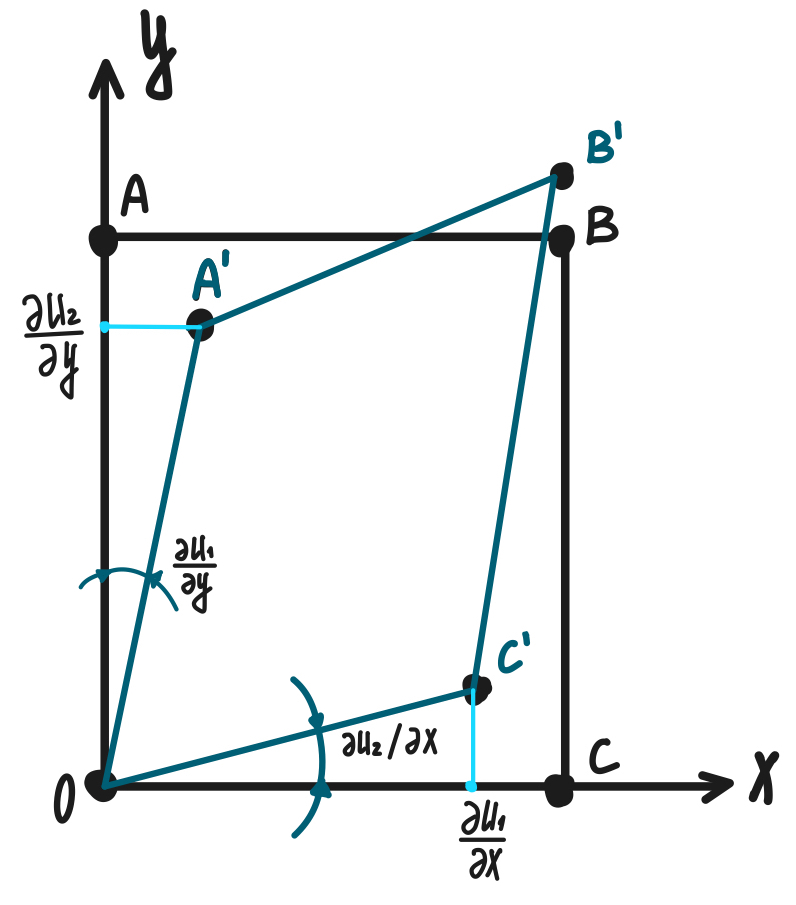
\includegraphics[width=0.6\textwidth]{deform.jpeg}
      \caption{Процесс деформации}
      \label{fig:deform}
    \end{figure}

    \pagebreak
    
    Используя все проделанные раннее рассуждения, преобразуем элемент расстояния $(dl^')^2$ к виду:
    \[
      \begin{split}
        (dl^')^2 &= (dl)^2 + 2 \displaystyle \sum_{k = 1}^{n} dx_k du_k + \displaystyle \sum_{j = 1}^{n} (du_k)^2 = (dl_i)^2 + 2 \displaystyle \sum_{k = 1}^{n} \displaystyle \sum_{l = 1}^{n} \dfrac{\partial u_k}{\partial x_l} dx_l dx_k \, + \\
        &+ \displaystyle \sum_{k = 1}^{n} \displaystyle \sum_{l = 1}^{n} \Bigl(\dfrac{\partial u_k}{\partial x_l} dx_l \Bigr)^2
      \end{split}
    \]

    Запишем в более лаконичном виде:
    \begin{equation}
      \begin{split}
        (dl^')^2 &= (dl)^2 + 2 \dfrac{\partial u_k}{\partial x_l} dx_l dx_k + \Bigl(\dfrac{\partial u_k}{\partial x_l} dx_l \Bigr)^2
      \end{split}
    \end{equation}

    При малых деформациях третьим слагаемым можно пренебречь в силу его большего порядка малости. 

    \pagebreak

    Во втором слагаемом индексы $j, k$ являются немыми, поэтому его можно записать в симметричном виде
    \begin{equation}
      \dfrac{\partial u_k}{\partial x_l} dx_l dx_k = \dfrac{1}{2} \Bigl( \dfrac{\partial u_k}{\partial x_l} + \dfrac{\partial u_l}{\partial x_k} \Bigr)dx_l dx_k = \varepsilon_{kl} dx_l dx_k,
      \label{deformTensorComponent}
    \end{equation}
    \noindent где $\varepsilon_{kl}$ -- составляющая тензора деформаций в точке $X$. 
    
    В предположении существования аддитивного разложения компонент тензора деформаций Коши запишем:
    \[
      \varepsilon_{kl} = \dfrac{1}{2}\Bigl( \dfrac{\partial u_k}{\partial x_l} + \dfrac{\partial u_l}{\partial x_k} \Bigr) = \varepsilon_{kl}^e +  \varepsilon_{kl}^0, \quad k, l = 1, 2, 3,
    \]
    \noindent где $\varepsilon_{kl}^e$ -- компоненты упругой состовляющей тензора деформаций, а $ \varepsilon_{kl}^0 $ -- компоненты тенхора неупругих деформаций среду (в нашем случае температурные деформации).
    
    Термоупругость описывает деформации при неравномерном нагреве деформируемых тел. Термоупругое тело обладает хотя бы одним естественным состоянием, в котором отсутствуют напряжения и деформации, при том температура во всех точках одинакова. Свяжем это состояние с начальной температурой тела $T_0$. При нагреве или охлаждении в теле возникают температурные деформации, описываемые тензором с компонентами $ \varepsilon_{kl}^0 \colon$
    \[
      \varepsilon_{kl}^0 = \alpha_{kl}^T \Delta T \Rightarrow \varepsilon_{kl}^0 \sim \alpha_{kl}^T,
    \]
    \noindent где $ \alpha_{kl}^T $ -- компоненты тензора теплового расширения.

    \subsection{Определяющее соотношение (закон Гука)}

    \section-{Заключение}
    
    \newpage

    \begin{thebibliography}{9}
  

    \end{thebibliography}

    \end{document}